\section{Experimental setup and measurements}
The setup and the way of measurement are based on \cite{anleitungV64}.
\label{sec:Experimentale}
The experiment is conducted by using the Sagnac-Interferometer introduced in \ref{subsec:Sagnac_Interferometer}. 
The topology of the interferometer can be seen in \autoref{pic:Sagnac-Interferometer}.As a 
source of light a Helium-Neon laser is used. The plane of the linearly polarized laser beam is tilted about $45°$ in comparison to 
the vertical. This leads to the beam being split into two beams of the same intensity and perpendicular polarization by the PBSC.
In front of the PBSC a polarization filter is placed so the incoming beam is traveling through the filter and afterwards through the 
PBSC. 

\begin{figure}
    \centering
    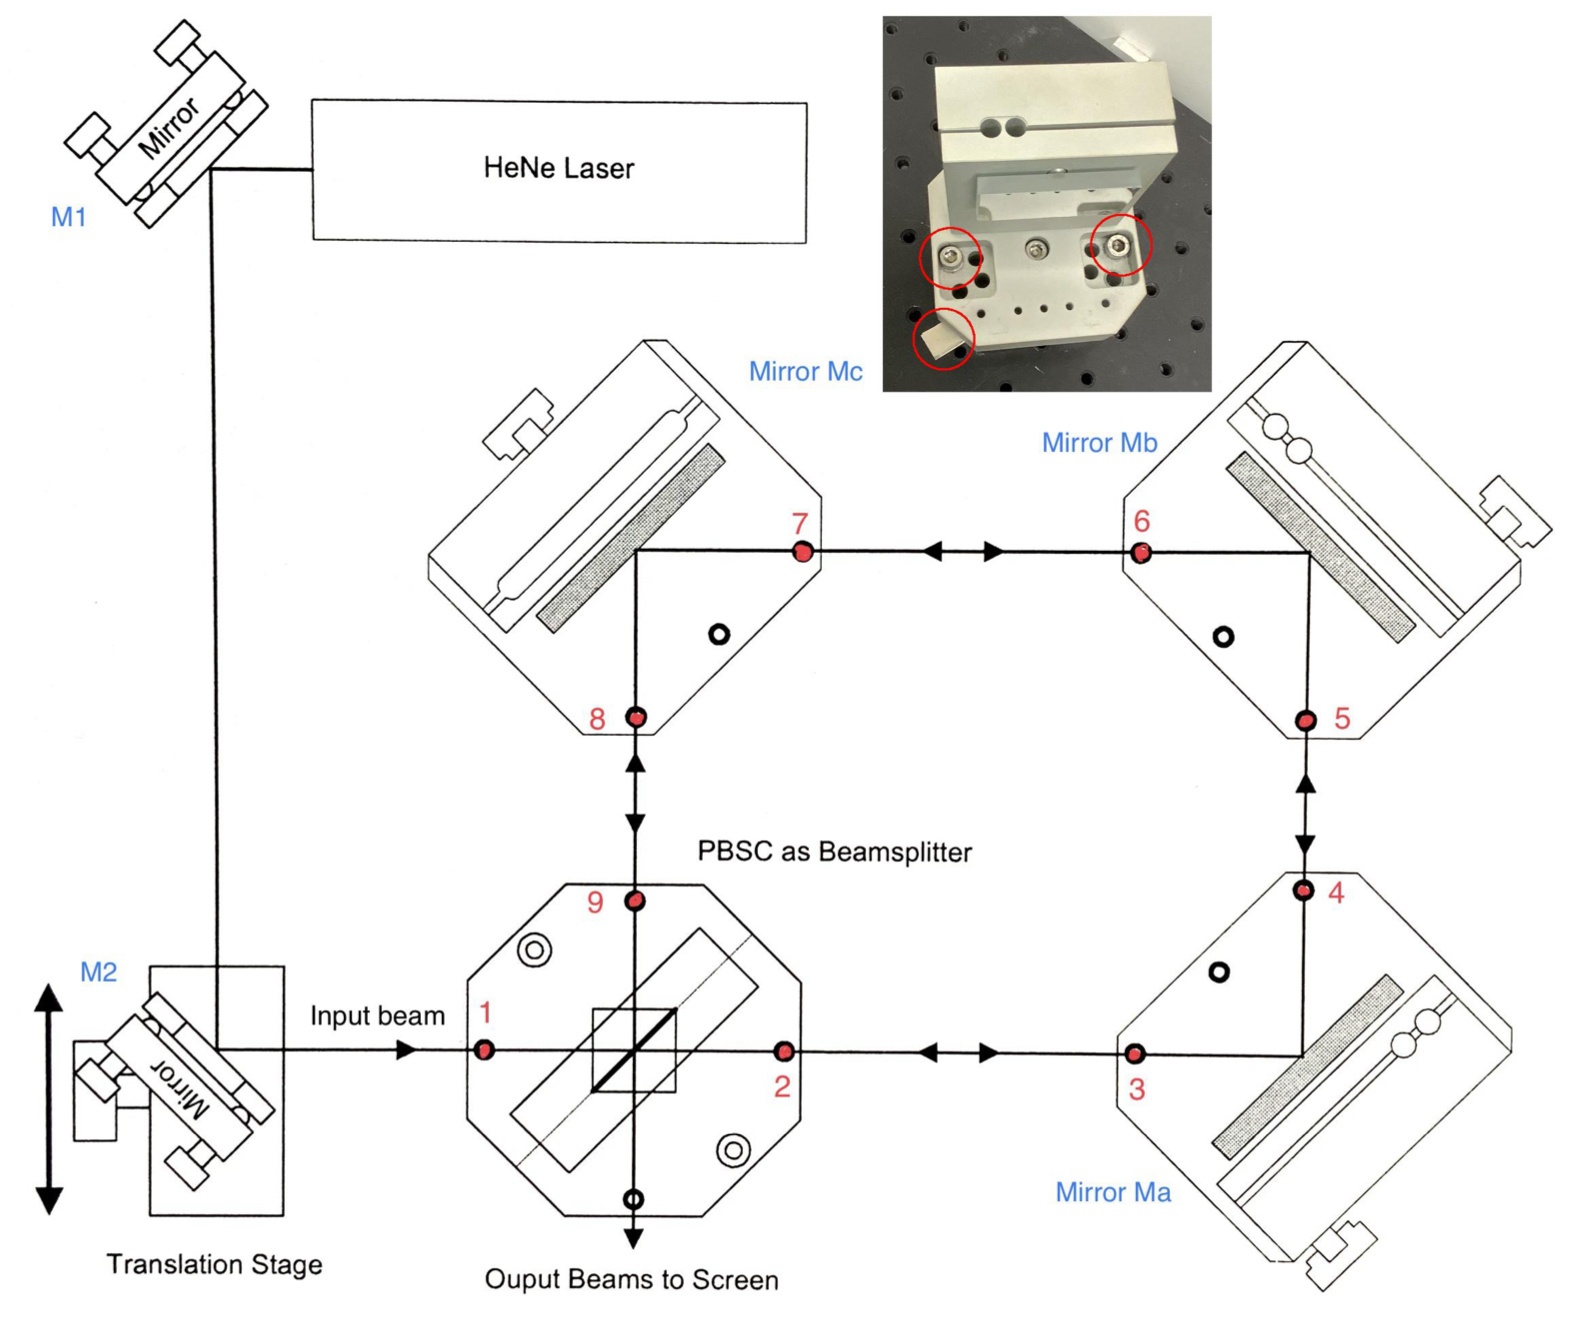
\includegraphics[width=0.70\textwidth]{content/Bilder/Sagnac_Interferometer.jpeg}
    \caption{Topology of the Sagnac-Interferometer \cite{anleitungV64}}
    \label{pic:Sagnac-Interferometer}
  \end{figure}

To make the interference of the two beams possible, the beams must travel through a polarization filter to create an overlapping polarization. 
At the end, the beam is led into two photodiodes. These diodes measure the brightness of the incoming beam. 

\subsection{Alignment}
The correct alignment is a critical part of the experiment. For the interference to work, the beams have to be parallel to each other and 
overlap at all times. This is achieved by using adjustment plates that have holes at the top where the beam should travel through. 
These can be put into the holes that are marked red on \autoref{pic:Sagnac-Interferometer}. The mirrors Ma and Mb can be adjusted horizontally
and the mirror Mc can be adjusted vertically. The mirrors M1 and M2 can be adjusted both vertically and horizontally. 
First the beam traveling from 
the PBSC to mirror Ma is calibrated by adjusting mirrors M1 and M2 alternately until the beam is able to pass through both holes on the 
adjustment plates on points 2 and 3. Then the beam traveling to mirror Mc is adjusted using the same method. After that mirror Mb
is adjusted in a way that the opposing beams meet at one single point on the PBSC. To be able to see an interference pattern behind the PBSC 
another polarization filter has to be installed at a 45° angle. The formed interference pattern can be used to determine if the two beams 
are really parallel to each other because otherwise some fringes will occur at the interference pattern. 

\subsection{Measurment of contrast}
First, the mirror M2 is moved so the incoming beam is parallel to the first surface PBSC. This separation of the two beams allows the beams 
to be manipulated individually. After that, a rotatable glass holder is installed between mirror Mc and the PBSC in the beam path. 
The holder contains two tilted glass plates that have a thickness of $d = \SI{1}{\milli\meter}$. The polarization filter at the end 
of the two beam paths is replaced by a PBSC, which is rotated by $45°$. One of the output beams of this PBSC is directed into a 
photodiode. To calculate the contrast, the maximal and minimal voltage of the diode is measured as a function of the angle of the 
polarization filter $\phi$. Per angle, the maximal and minimal voltage is recorded three times. The measurement is taken in a range 
of $0° - 180°$ for $\phi$ in $10°$ steps. The maximal and minimal voltage is achieved by rotating the glass holder. 
For the following parts of the experiment, the polarization filter is set to the angle that produces the highest contrast and the 
highest intensity. 

\subsection{Refractive index of glass}
To measure the refractive index of glass, now both beams are directed into one photodiode each. To reduce noise the voltage difference 
between the two photodiodes is measured instead of the absolute values. Then the glass is rotated ten times by $10°$ and the number of 
maxima (or minima) is counted each time.

\subsection{Refractive index of air}
For this part of the experiment, a gas cell of the length $L = \SI{100}{\milli\meter}$ is inserted into the path of one beam. Then the 
gas cell is evacuated using a vacuum pump and then gradually refilled with air. Every $\SI{50}{\milli\bar}$ the number of maxima (or minima)
is noted until ambient pressure is reached. This measurement is taken three times. 

